\section{Avvio e monitoraggio del servizio di Bake}
\label{sec:chapter_caso_uso_section_2}

In qualsiasi momento, durante la creazione della scena nell’editor, l’utente può decidere di avviare il processo di bake.
L’utente deve prima compilare i campi relativi al nome del processo di bake, il valore di sample e la mail dove verrà inviato il risultato di bake.
Una volta inseriti i campi, l’utente preme il pulsante bake ed avvia il servizio in remoto.
I servizi avviati possono essere monitorati tramite il pulsante \emph{JOBS}.
\\
L’utente a questo punto attende la notifica tramite mail del completamento del servizio.
Durante l’attesa può continuare a creare altre scene tramite l’editor, oppure monitorare i processi di bake lanciati tramite il pulsante \emph{JOBS}.
\\
Questo pulsante mostra nel pannello tutti i servizi avviati, permettendo di interagire con essi. \\
Per ogni servizio mostrato vengono infatti associati due ulteriori messaggi.
Per ogni processo è possibile richiedere lo \emph{status}, tramite il corrispondente pulsante, utile ad informare l’utente del completamente del job richiesto tramite differenti messaggi:
\begin{itemize}
\item La percentuale di completamento se il processo è in esecuzione.
\item Il numero di processi in coda se il processo è in attesa di essere eseguito.
\item Sollecita di lettura mail se il processo è terminato.
\end{itemize}
Inoltre in qualsiasi momento l’utente può decidere di cancellare un processo tra quelli avviati tramite il pulsante \emph{delete}.
\\
\begin{figure}[htb]
 \centering
 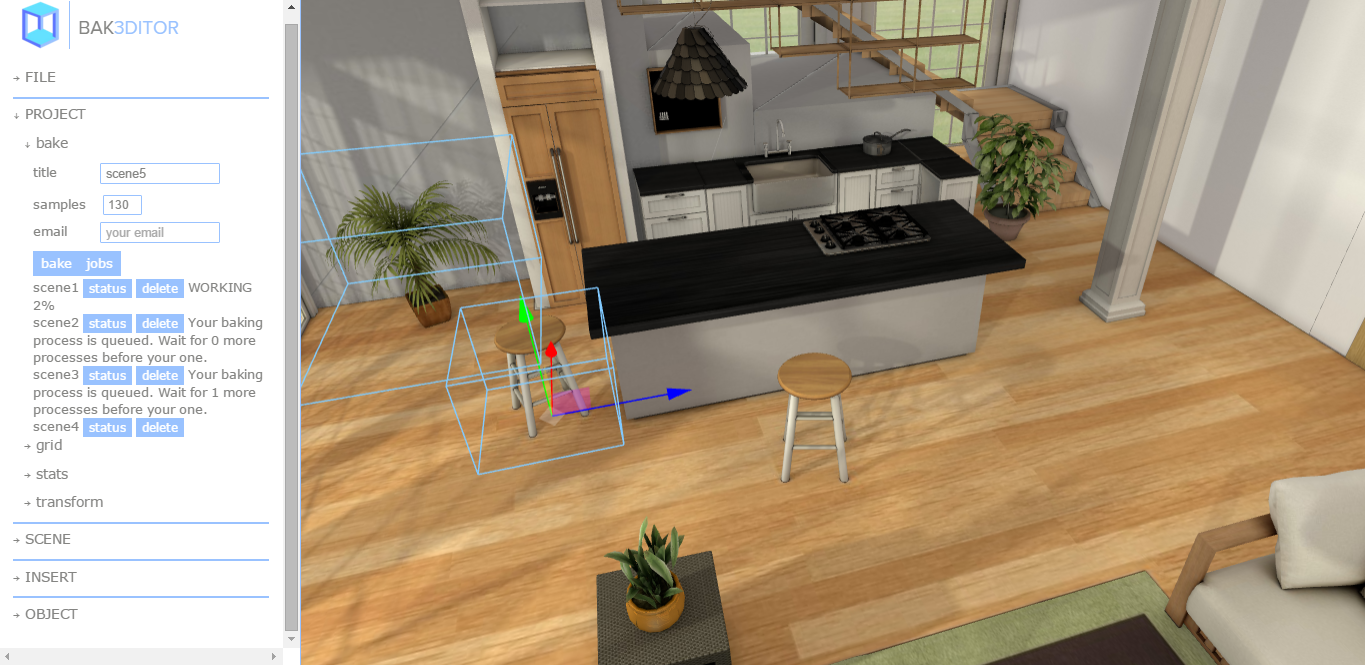
\includegraphics[width=1\linewidth]{images/chapter_caso_uso/service_bake.png}\hfill
 \caption[Pannello di interazione con il servizio]{Il pannello per interagire con il servizio Bake}
 \label{fig:caso_uso_service_bake}
\end{figure}